\documentclass[a4paper]{article}

\usepackage{algorithm,amsmath,amssymb,subfig,url}
\usepackage[pdftex]{graphicx}
\usepackage[margin=30mm]{geometry}
\usepackage[format=hang,labelfont=it]{caption}
\usepackage[noend]{algorithmic}

\floatname{algorithm}{Listing}
\algsetup{indent=3em}
\renewcommand{\algorithmiccomment}[1]{\quad \{\emph{#1}\}}



\begin{document}
\title{
  \large
  DT8014 Algorithms Group Activities (2014)\\
  \Large
  Week 3 -- Selected Graph Problems}
\author{Roland Philippsen}
\maketitle



\noindent
Form groups of 4-5 students and work together on the following tasks.


\section*{Working with Graph Properties}

\emph{Purpose: gain a deeper understanding of some graph concepts.}

\vspace{\baselineskip}
\noindent
\textbf{Team Ace of Spades}
\begin{enumerate}
\item
  Draw a 2-connected simple graph, and a planar graph with a 4-clique.\\
  \emph{After 5 minutes, present your examples on the whiteboard.}
\item
  Sketch an algorithm that determines whether a given graph is bipartite.\\
  \emph{After 10 minutes, present your algorithms on the whiteboard.}
\end{enumerate}

\vspace{\baselineskip}
\noindent
\textbf{Team Ace of Clubs}
\begin{enumerate}
\item
  Draw all planar bipartitie graphs where one of the two vertex sets contains 3 vertices and each vertex from one set is adjacent to all the vertices of the other.\\
  \emph{After 5 minutes, present your examples on the whiteboard.}
\item
  Sketch an algorithm that determines whether a given graph is 2-connected.\\
  \emph{After 10 minutes, present your algorithms on the whiteboard.}
\end{enumerate}
  
\vspace{\baselineskip}
\noindent
\textbf{Team Ace of Hearts}
\begin{enumerate}
\item
  Draw a simple 4-regular graph whose maximal clique size is 4.\\
  \emph{After 5 minutes, present your example(s) on the whiteboard.}
\item
  Sketch an algorithm that determines whether a given graph is bipartite.\\
  \emph{After 10 minutes, present your algorithms on the whiteboard.}
\end{enumerate}

\vspace{\baselineskip}
\noindent
\textbf{Team Ace of Diamonds}
\begin{enumerate}
\item
  Draw a non-planar graph whose maximal clique size is 2.\\
  \emph{After 5 minutes, present your example(s) on the whiteboard.}
\item
  Sketch an algorithm that determines whether a given graph is 2-connected.\\
  \emph{After 10 minutes, present your algorithms on the whiteboard.}
\end{enumerate}


\clearpage
\section*{Minimum Spanning Tree}

\emph{
  Purpose: become familiar with a widely applicable graph problem, and encounter a greedy algorithm which is known to be optimal.
}

Given a connected, undirected graph, a \textbf{spanning tree} of that graph is a subgraph that is a tree and connects all the vertices together.
A given graph can have many different spanning trees.
We can also assign a weight to each edge, which is a number representing how unfavorable it is, and use this to assign a weight to a spanning tree by computing the sum of the weights of the edges in that spanning tree.
A \textbf{minimum spanning tree (MST)} or minimum weight spanning tree is then a spanning tree with weight less than or equal to the weight of every other spanning tree.

\begin{enumerate}

\item
  Describe two real-world problems which can be modeled such that an MST solves them.
  
\item
  Sketch a proof for the uniqueness property:\\
  \emph{If each edge has a distinct weight then there will be only one, unique minimum spanning tree.}
  
\item
  Sketch a naive brute-force approach for computing the MST.
  By now, this shouldn't take you more than two or three minutes\ldots
  
\item
  Apply Kruskal's algorithm, given in Listing~\ref{algo:kruskal}, to find the MSTs for the graphs in Figure~\ref{fig:mst-exercise}.

\end{enumerate}



\begin{algorithm}
  \caption{
    Kruskal's Algorithm\\
    \textbf{Input:} an undirected weighted graph $G=(V,E)$\\
    \textbf{Relies on} a disjoint-set data structure:\\
    -- MakeSet($v$) makes a set containing a single element $v$.\\
    -- FindSet($v$) determines the set which contains a given element.\\
    -- Union($u,v$) joins the subsets to which two given elements belong.
  }\label{algo:kruskal}
  \begin{algorithmic}
    \STATE $A \leftarrow \varnothing$
    \FORALL {$v \in V$}
      \STATE MakeSet($v$)
    \ENDFOR
    \STATE $S \leftarrow$ all edges $(u,v) \in E$ sorted by increasing weight.
    \FORALL {$(u,v) \in S$}
      \IF {FindSet($u$) $\ne$ FindSet($v$)}
        \STATE $A \leftarrow A \cup \{(u,v)\}$
        \STATE Union($u,v$)
      \ENDIF
    \ENDFOR
    \RETURN $A$
  \end{algorithmic}
\end{algorithm}

\begin{figure}[H]
  \centering
  \subfloat[]{
    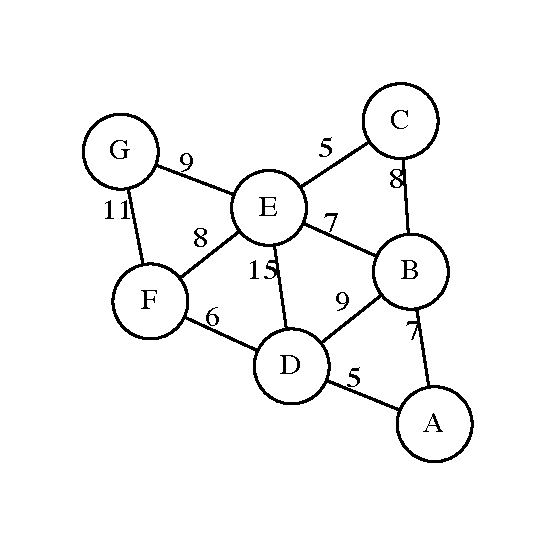
\includegraphics[width=0.3\columnwidth,trim=1cm 1cm 1cm 1cm]{fig/mst-exercise-1.pdf}}
  \hspace{15mm}
  \subfloat[]{
    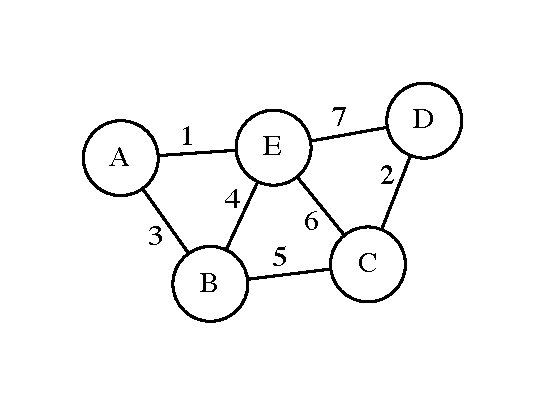
\includegraphics[width=0.3\columnwidth,trim=1cm 1cm 1cm 1cm]{fig/mst-exercise-2.pdf}}
  \caption{
    Example weighted undirected graphs.
  }\label{fig:mst-exercise}
\end{figure}


\end{document}
